\chapter{Advertising and Pricing: Fixed Prices}

The goal of this final part is the maximization of the total reward by attracting the most valuable users through the Advertising algorithms in a scenario where it is not possible to choose a different price for each class of user. In this scenario, differently from what we have seen in chapter 6, we have the further constraint that the seller charges a unique price to all the classes of users and so we cannot find what is the best price for each subcampaign as we did before, but we have to find a \textit{single optimal price} able to maximize the revenue for all the subcampaigns.\\ In the following sections we go through the reward maximization algorithms we implemented to choose the best price for all the users that together with the Adverting will bring the best possible reward.


\section{Proposed Integration}
The main idea to solve the described problem is to iterate over all the possible prices in order to choose the one that jointly with the corresponding advertising optimization will produce the best reward.
To achieve this goal we updated the \textit{Budget Allocator} implemented in part 6 which in this new scenario iterates over all the possible prices and thanks to the information received by the \textit{Sub Campaign Handlers} \footnote{The Sub Campaign Handler is a component in charge to learn both the advertising curve and the demand curve associated to a specific sub campaign} it computes the best budget allocation which will be used jointly to the price to estimate the corresponding number of purchases and relative revenue. At the end of this iteration the Budget Allocator will choose the optimal price, that is the one with the greatest estimated reward and it will propose it to the users the next day combined with the already computed allocation for the advertising sub campaigns.\\ This problem has been tackled with two different approaches, the first one based on a \textit{Bernoulli} model, while the second one based on a \textit{Normal} model. Both implementations will be better described in the following sections. \\It is important to remark that also in this scenario the main idea was to decompose, wherever feasible, the two problems, namely the Advertising and Pricing, in order to reuse as much as possible all the algorithms presented in the previous chapters.


\section{First implementation: based on Bernoulli distribution}
In our first implementation we approached the Pricing problem exploiting the algorithm already implemented for the previous problems. More precisely in this implementation every time a new user enters on the website, the Environment determines if she will buy or not the item, by making an extraction from a \textit{Bernoulli distribution}. Under this assumption we could reuse the \textit{Thompson Sampling} algorithm already implemented for solving the pricing problem on Part 4.
On the other hand to learn the Advertising curves associated to each subcampaign we used the GPTS already implemented for solving the Advertising subproblem as we did in part 6.\\ The performance of the implemented algorithm is for now postponed and it will be analyzed in the last section, after the description of the second approach we went through.


\section{Second implementation: based on Normal distribution}
For the second implementation we started from the consideration that under certain constraints the binomial distribution is well approximated by the normal distribution. Let's consider the binomial distribution defined by the function:
\begin{equation}
    f(x) = \binom{n}{x}  p^x q^{n-x}
\end{equation}

which represents the probability of exactly $x$ successes in $n$ independent Bernoulli trials where a given trial has two possible outcomes, that is a "success" and a "failure"\footnote{In our scenario a success is when the user purchases the item once he visits the website, while a failure if she doesn't} respectively with probability $p$ and $q=(1-p)$.\\ When $n$, $np$ and $nq$ are large, then the binomial distribution is well approximated by the normal distribution:
\begin{equation}
    f(x)  \sim \frac{1}{\sqrt{2 \pi npq}} e^{ \frac{-(x-np)^2}{2npq} }
\end{equation}

Since we are working with very large value of $n$, we can proceed with such approximation without worrying about the value of $np$ and $nq$.
So we can consider the case in which the pricing Environment is based on a \textit{Normal distribution}. Under these considerations, all the information are collected at the end of the day and no more at each visit. In this way the number of purchases will be considered as an aggregation of Bernoulli extractions.
In this second implementation the curves associated to the Pricing and Advertising subproblems are both learned by using the GPTS algorithm already implemented.\\
Differently from the previous implementation in which we collected the information after each visit of a user, in this case we learn the approximated distribution and so we could have more problems with suboptima. To solve this problem we have introduced the concept of \textit{artificial fading}\footnote{The noise decreases linearly as the number of days increases} \textit{noise}, i.e. a random noise added to the confidence of the arms once they are pulled. Indeed using the Gaussian Process to learn the curves we have more problems to find the best solution to the exploration-exploitation trade-off dilemma because we have more possibilities to discard the true optimal arm. By adding this fictitious noises we will increase the exploration phase and in this way we avoid that the algorithm focuses on a suboptimum.\\ It is important to remark that,since we use the GPTS algorithm to solve both the Pricing and Advertising subproblems, the noise has to be added to both the curves learned by the corresponding learners.\\ During the performance evaluation in the next section we will compare the behavior of this implementation with respect to the first one and we will analyze the difference we have by running this algorithm with and without the artificial noises.


\section{Performance Evaluation}
This section aims to compare and describe the performances of the above described algorithms. In Fig. \ref{regretPart7Binomial} we can see the regret associated to the first described algorithm, that is in the case in which the Environment make an extraction from a Bernoulli distribution every time a new user visits the page.

\begin{figure}
    %\captionsetup{justification=centering,margin=1cm}
    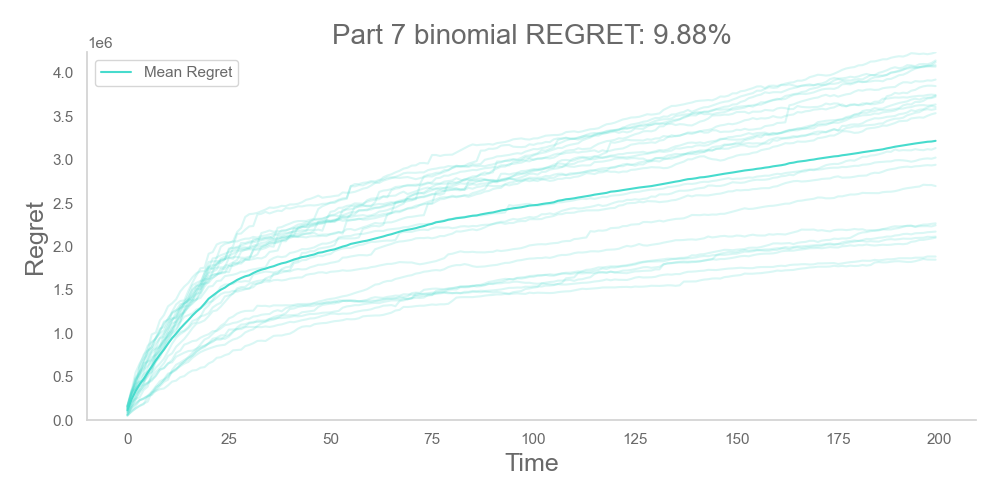
\includegraphics[width=\textwidth]{images/part7_binomial_regret.png}
    \caption{Regret obtained when we consider an Environment which makes Bernoulli extractions.}
    \label{regretPart7Binomial}
\end{figure}

In Figure \ref{fig:RegretsPart7Normal} we show the regret associated to the second implementation, that is in the case in which the Environment collects the information from an approximated Normal distribution. In the figure we can also see how, in this scenario, the performance changes varying the value of the artificial noises.

\begin{figure}[!htb]
    \centering

    \begin{subfigure}[!H]{0.8\textwidth}
        \centering
        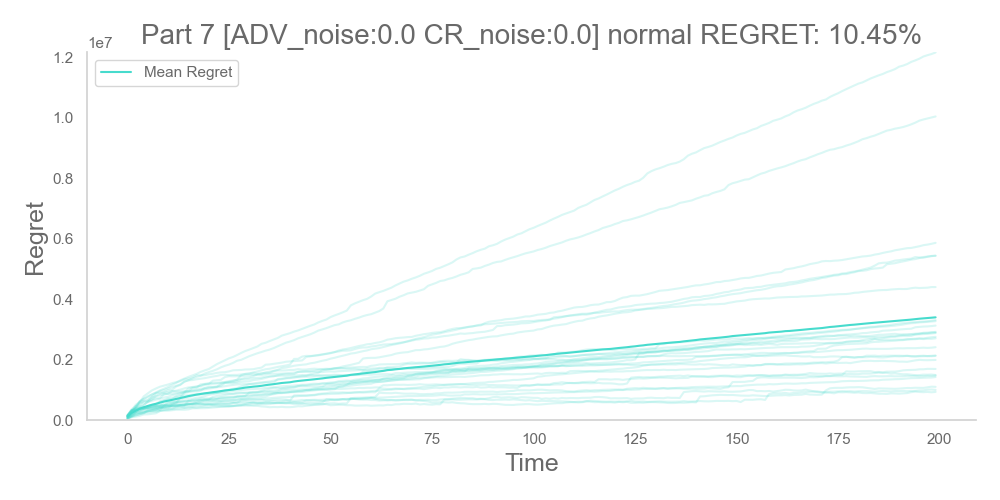
\includegraphics[width=\textwidth]{images/part7_normal_regret_noise00.png}
        \caption{Regret without artificial noise.}
    \end{subfigure}

    \begin{subfigure}[!H]{0.8\textwidth}
        \centering
        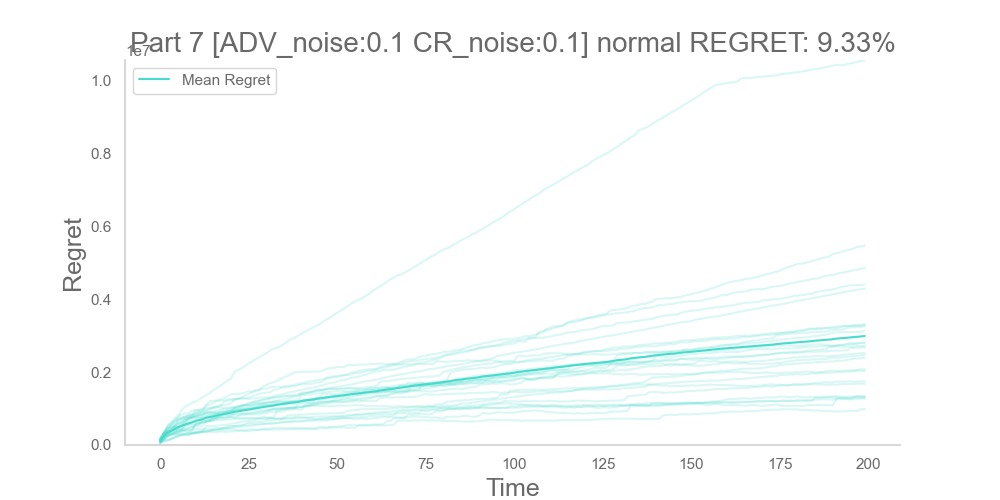
\includegraphics[width=\textwidth]{images/part7_normal_regret_noise01.jpeg}
        \caption{Regret with artificial noise equal to 0.1.}
    \end{subfigure}

    \begin{subfigure}[!H]{0.8\textwidth}
        \centering
        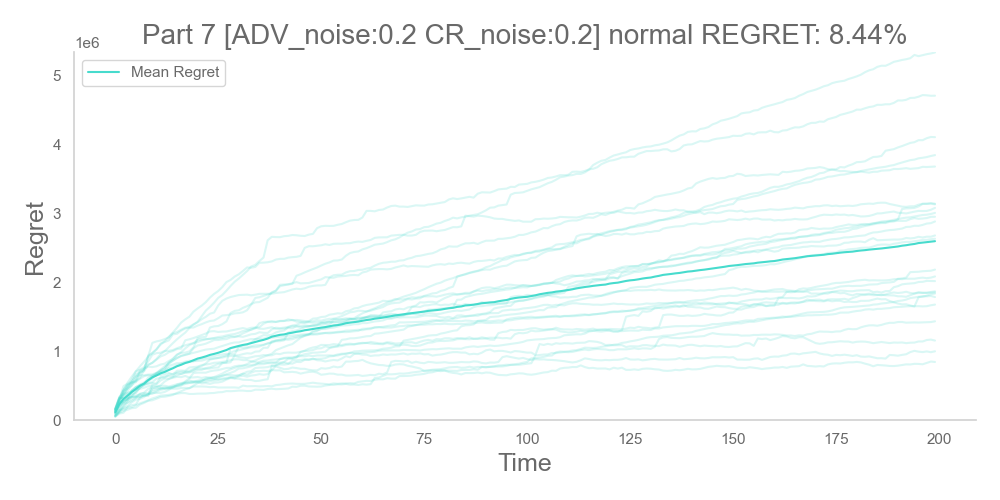
\includegraphics[width=\textwidth]{images/part7_normal_regret_noise02.png}
        \caption{Regret with artificial noise equal to 0.2.}
    \end{subfigure}

    \caption{Comparison between the regrets with and without the artificial noises when we consider an Environment based on a Normal distribution.}
    \label{fig:RegretsPart7Normal}
\end{figure}